\documentclass{beamer}
\usepackage[utf8]{inputenc}
\usepackage[english]{babel}
\usepackage{amsmath}
\usepackage{amssymb}
\usepackage{fancyhdr}
\usepackage{pgfplots}
\usepackage{setspace}
\usepackage{listings}
\pgfplotsset{compat=1.17} 
\usepackage{enumerate}
\usepackage{algorithm}
\usepackage{algpseudocode}
% \geometry{a4paper} % or letter or a5paper or ... etc
% \geometry{landscape} % rotated page geometry
% \usepackage[margin=2cm]{geometry}
\usepackage{minted}
\usepackage[most]{tcolorbox}
\newtcolorbox{tb}[1][]{%
  sharp corners,
  enhanced,
  colback=white,
  height=6cm,
  attach title to upper,
  #1
}

%These setting will make the code areas look Pretty
\lstset{
	escapechar=~,
	numbers=left, 
	%numberstyle=\tiny, 
	stepnumber=1, 
	firstnumber=1,
	%numbersep=5pt,
	language=C,
	% stringstyle=\itfamily,
	%basicstyle=\footnotesize, 
	showstringspaces=false,
	frame=single,
  upquote=true
}

% created 2022-May-23 %
% Theme choice:
\usetheme{AnnArbor}
% Title page details: 
\title{Memory in C}
\author{Jonathan Parlett}
\date{\today}

\begin{document}

% Title page frame
\begin{frame}
    \titlepage
\end{frame}

\begin{frame}{Memory}
	A big part of C is memory management, so lets discusses how memory is relevant to programs.

	\begin{itemize}
		\item Each program has a section of memory allocated to it by the operating system when it is executed. 
		\item If a program attempts to access another programs memory space a segmentation fault occurs and the program is terminated.
		\item The operating system is also a program, and there is a section of memory that is owns.
	\end{itemize}
\end{frame}

\begin{frame}{Stack and Heap}
	Each section of memory allocated to a C program by the operating system is divided into the {\bf Stack} and the {\bf Heap}.

	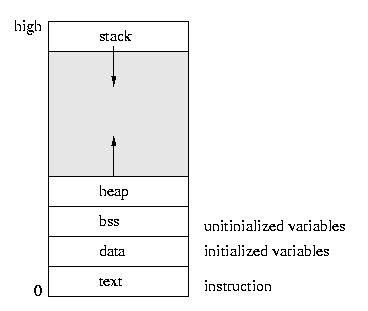
\includegraphics[scale=0.40]{imgs/stackandheap.jpeg}

	Stack memory is managed for you. Whenever you are declaring variables, arrays, or instances of structs, they are located on the stack.
\end{frame}

\begin{frame}{Stack and Heap}
	\begin{itemize}
	\item Anything allocated on the stack is also reclaimed automatically, when the program terminates or things fall out of scope. local variables of a function are reclaimed when the function returns for example.

	\item Whenever you are using {\it malloc()} to get space for a structure or variable you are using memory on the heap. This memory once allocated will not be reclaimed until you reclaim it. It is within your control.
	\end{itemize}
\end{frame}

\begin{frame}{Static vs Dynamic Memory}
	\begin{itemize}
		\item Static or compile time memory is the memory that is managed for you. It again uses the stack. This is managed by the compiler and since items are statically declared in the code we say it is allocated at compile time.

		\item Dynamic memory is again the memory that you manage. It is allocated by calls to {\it malloc()}. So it allocated programmatically during execution execution, so it is also called run time memory allocation.
	\end{itemize}
\end{frame}

\begin{frame}{Memory as a Table}
	We can think of memory as a $n$x2 table. The indices of the table are memory addresses (just numbers), and the data at each row is the value stored in that memory location. For now this is a simplified table. We will ignore the relevance of the sizes of data types, and consider each row a single item of type {\it int}.

	\begin{tabular}{|c|c|}
		\hline
		Address & Data\\
		\hline
		0 & 55 \\
		\hline
		1 & 49 \\
		\hline
		\vdots & \vdots \\
		\hline
		n & 13\\
		\hline
	\end{tabular}

A pointer holds a table index (memory address). So if 49 is stored at location 1 then a pointer to 49 would have the value 1. From this it should be clear that memory addresses are just numbers, so the values of pointers are just numbers. To clarify the value {\bf at} pointers is a different matter, but in C pointers are just 64 bit integers.
\end{frame}

\begin{frame}[fragile]{Pointer Operations: Address Of (\&)}
	Again consider the memory table.

	\begin{tabular}{|c|c|}
		\hline
		Address & Data\\
		\hline
		0 & 55 \\
		\hline
		1 & 49 \\
		\hline
		\vdots & \vdots \\
		\hline
		n & 13\\
		\hline
	\end{tabular}

	Given a data item in our table, the address of (\&) operator gives us the index (memory address) of our data item;

\begin{minted}[frame=lines]{c}
int i = 49; //corresponds to row 1
printf("location of i: %d\n", &i); //prints 1
\end{minted}
In effect {\it \&i} gives us a pointer to {\it i}.

\end{frame}

\begin{frame}[fragile]{Pointer Operations: Dereference (*)}
A pointer holds a table index (memory address). When we dereference said pointer we are retrieving the item at that index.

\begin{tabular}{|c|c|}
		\hline
		Address & Data\\
		\hline
		0 & 55 \\
		\hline
		1 & 43 \\
		\hline
		2 & 8 \\
		\hline
		\vdots & \vdots \\
		\hline
		n & 13\\
		\hline
	\end{tabular}
\begin{minted}[frame=lines]{c}
//pointer holds index 2
int* i = 2;
//dereferencing (*), and printing value at row 2 <-> 8
printf("value at i: %d\n", *i);
\end{minted}
\end{frame}

\begin{frame}[fragile]{Pointer Operations: Addition (+)}
Arrays are one of the most basic data structures, they are simply a collection of contiguous memory locations. So all elements are placed one after the other in memory.
\mint{c}|int A[5] = {1,2,3,4,5}|
Arrays are pointers. The value of $A$ is just a memory address. lets say its 113. Then the array corresponds to the following mem table.
\begin{tabular}{|c|c|}
		\hline
		Address & Data\\
		\hline
		0 & 55 \\
		\hline
		\vdots & \vdots \\
		\hline
		113 & 1\\
		\hline
		114 & 2 \\
		\hline
		115 & 3 \\
		\hline
		116 & 4 \\
		\hline
		117 & 5 \\
		\hline
		\vdots & \vdots \\
		n & 13\\
		\hline
	\end{tabular}

\end{frame}

\begin{frame}[fragile]{Pointer Operations: Addition (+)}
\begin{tabular}{|c|c|}
		\hline
		Address & Data\\
		\hline
		0 & 55 \\
		\hline
		\vdots & \vdots \\
		\hline
		113 & 1\\
		\hline
		114 & 2 \\
		\hline
		115 & 3 \\
		\hline
		116 & 4 \\
		\hline
		117 & 5 \\
		\hline
		\vdots & \vdots \\
		n & 13\\
		\hline
	\end{tabular}

	We can add to pointers just like we can add to integers. It functions slightly differently for reasons that well expand on shortly, but consider in our current diagram we can access every element of our array, by adding its index in the array to $A$ and dereferencing the result like so {\it *(A+i)}.
\end{frame}

\begin{frame}[fragile]{Pointer Operations: Addition (+)}
	Lets explore some code to confirm this is how it works.
\begin{minted}[frame=lines, fontsize=\footnotesize]{c}
int A[5] = {6,7,8,9,10};

printf("Val of base pointer A = 0x%x\n", A);

printf("________________________________________________________\n");
for(int i=0; i < 5; i++){
	printf("*(A+%d) = %d | ", i, *(A+i));
	printf("A[%d] = %d | ", i, A[i]);
	printf("Address of value at (A+%d) = 0x%x\n", i, (A+i));
}
\end{minted}
\end{frame}

\begin{frame}[fragile]{Pointer Operations: Addition (+)}
Our output should look something like, only the values of $(A+i)$ will differ.
\begin{minted}[frame=lines, fontsize=\footnotesize]{c}
Val of base pointer A = 0x388e5690
______________________________________________________________
*(A+0) = 6 | A[0] = 6 | Address of value at (A+0) = 0x388e5690
*(A+1) = 7 | A[1] = 7 | Address of value at (A+1) = 0x388e5694
*(A+2) = 8 | A[2] = 8 | Address of value at (A+2) = 0x388e5698
*(A+3) = 9 | A[3] = 9 | Address of value at (A+3) = 0x388e569c
*(A+4) = 10 | A[4] = 10 | Address of value at (A+4) = 0x388e56a0
\end{minted}
Everything seems to make sense, dereferencing $(A+i)$ gets us the ith element same as $A[i]$, but look at how $(A+i)$ increases in value. It increments by 4 each time instead of 1, like our current memory model would cause us to expect.
\end{frame}

\begin{frame}[fragile]{The type system}
To understand why this happens we need to understand a little bit about the type system and the sizes of different types.
\begin{itemize}
	\item The atomic unit of memory in C is the {\bf byte} (8 bits).
	\item Each type in C takes up a certain amount of {\bf bytes} of memory.
	\item The function {\it sizeof()} takes either a type or variable as an argument.
	\item Given a type {\it sizeof()} returns the size of the type in bytes, and given a variable it returns the size of the type of the variable in bytes. It does {\bf not} return the size of an array. Given an array it will just return the size of the type which is a pointer.
\end{itemize}
\end{frame}

\begin{frame}[fragile]{The type system}
Lets look at the size of some types. Please be aware that sizes may be different on different hardware platforms, so these may not be same on your system.

\begin{minted}[frame=lines, fontsize=\footnotesize]{c}
printf("Size of integer = %lu\n", sizeof(int));                             //prints 4 (4 bytes = 32 bits)
printf("Size of long integer = %lu\n", sizeof(long int));                   //prints 8
printf("Size of unsigned long integer = %lu\n", sizeof(unsigned long int)); //prints 8
printf("Size of size_t = %lu\n", sizeof(size_t));                           //prints 8
printf("Size of char = %lu\n", sizeof(char));                               //prints 1
//these will all print 8
printf("Size of int* = %lu\n", sizeof(int*));
printf("Size of char* = %lu\n", sizeof(char*));
\end{minted}
Observe that an integer is 4 bytes, also that all pointers are the same size. Again pointers are just numbers, specifically in C they are unsigned 64 bit integers. Thus all pointers regardless of type have the same size of 8 bytes.
\end{frame}

\end{document}
